%
% File acl2020.tex
%
%% Based on the style files for ACL 2020, which were
%% Based on the style files for ACL 2018, NAACL 2018/19, which were
%% Based on the style files for ACL-2015, with some improvements
%%  taken from the NAACL-2016 style
%% Based on the style files for ACL-2014, which were, in turn,
%% based on ACL-2013, ACL-2012, ACL-2011, ACL-2010, ACL-IJCNLP-2009,
%% EACL-2009, IJCNLP-2008...
%% Based on the style files for EACL 2006 by 
%%e.agirre@ehu.es or Sergi.Balari@uab.es
%% and that of ACL 08 by Joakim Nivre and Noah Smith

\documentclass[11pt,a4paper]{article}
\usepackage[hyperref]{acl2020}
\usepackage{booktabs}
\usepackage{graphicx}
\usepackage{times}
\usepackage{latexsym}
\usepackage{enumitem}
\usepackage{subcaption}
\renewcommand{\UrlFont}{\ttfamily\small}

\usepackage{microtype}

\aclfinalcopy % Uncomment this line for the final submission


\newcommand\BibTeX{B\textsc{ib}\TeX}

\title{Fake News Detection and Source Credibility Analysis}

\author{Yongbo Chen \\
  Tulane University / New Orleans, LA \\
  \texttt{ychen88@tulane.edu} \\\And
  Nazmun Nahar Khanom \\
  Tulane University / New Orleans, LA \\
  \texttt{nkhanom@tulane.edu} \\}

\date{}

\begin{document}
\maketitle
% \begin{abstract}
% Lorem ipsum dolor sit amet, consectetur adipiscing elit, sed do eiusmod tempor incididunt ut labore et dolore magna aliqua. Ut enim ad minim veniam, quis nostrud exercitation ullamco laboris nisi ut aliquip ex ea commodo consequat. Duis aute irure dolor in reprehenderit in voluptate velit esse cillum dolore eu fugiat nulla pariatur. Excepteur sint occaecat cupidatat non proident, sunt in culpa qui officia deserunt mollit anim id est laborum.
% \end{abstract}


\section{Problem Overview}

With the rapid advancement of social media, misinformation and fake news increasingly threaten societal trust and stability. 
Due to inadequate verification methods, fake news spreads quickly across digital platforms, significantly impacting public opinion, political decisions, and public safety. 
Given the impracticality of manual fact-checking at scale, we propose a comprehensive fake news detection system using Natural Language Processing (NLP) techniques, 
integrating text classification, Named Entity Recognition (NER), and stance detection to systematically evaluate news reliability.

\section{Data Overview}

At the beginning, we planned to utilize the widely recognized FakeNewsNet dataset \cite{shu2018fakenewsnet, shu2017fake, shu2017exploiting} as our primary source of data for implementing our fake news detection system. However, we observed that FakeNewsNet only contains news titles and URLs, which are sufficient for basic classification tasks but insufficient for conducting more advanced analyses, such as Named Entity Recognition (NER) and stance detection as we planned.

Therefore, we selected an alternative dataset, called the Fake News Detection Datasets \cite{ahmed2018detecting, ahmed2017detection}, publicly available on Kaggle, a widely popular platform for datasets storage and sharing. This dataset encompasses two distinct types of news articles pre-labeled as fake and genuine. In more deails, it consists of two primary CSV files:

\begin{itemize}
    \item \texttt{True.csv}: Contains more than 12,600 genuine news articles sourced from Reuters.com.
    \item \texttt{Fake.csv}: Contains more than 12,600 fake news articles gathered from various unreliable platforms.
\end{itemize}

For our implementation, we programmatically downloaded this dataset through the Kaggle API into our local development environment. Additionally, to facilitate effective model training and evaluation, we divided the dataset into training and testing subsets with an 8:2 split ratio.

\section{Method}

\subsection{Implementation Pipeline}

Our approach involves a multi-step Natural Language Processing (NLP) pipeline including the steps of text preprocessing, feature extraction, classification modeling, and Named Entity Recognition (NER).

\textbf{Text Preprocessing:} We initiate our pipeline with standard preprocessing steps to clean and normalize the textual data. 
These steps include tokenization, stopword removal, stemming, and lemmatization. Specifically, we use the spaCy library for the tokenization and lemmatization, 
and the NLTK library for stopword filtering.

\textbf{Feature Extraction:} Our priority chose of model is using the BERT. Considering the original BERT model has already provided powerful deep contextual embeddings, 
we directly we directly leverage BERT's built-in contextual embeddings by fine-tuning the pre-trained BERT model (\texttt{bert-base-uncased}) available through Hugging Face's Transformers library \cite{DBLP:journals/corr/abs-1810-04805}. 
However, since one of our evaluation goal is to compare with other base models, we are still going to apply other feature extraction methods like TF-IDF or traditional word embeddings like Word2Vec during our implementation. 

\textbf{Named Entity Recognition (NER):} Initially, our model was only able to classify news articles as fake or real. To enhance its ability to detect misinformation, we integrated Named Entity Recognition (NER). 
To perform NER, we used the dbmdz/bert-large-cased-finetuned-conll03-english model from the Hugging Face Transformers library \cite{dbmdz_bert_large_cased_conll03}. This model excels at identifying and categorizing named entities, and the entity counts (e.g., the number of people, organizations, and locations) were added as additional features to our dataset.

\textbf{Classification Model:} Our core classification approach centers on fine-tuning the pre-trained BERT transformer specifically tailored to detect fake news. 
As mentioned above, we utilized the base BERT model (\texttt{bert-base-uncased}) provided by Hugging Face and employ a supervised learning methodology to fine-tune the model to accurately classify news articles as either fake or true.

\subsection{Evaluation}
After the previous implementation, we want to run several experiments to evaluate our model from several aspects. Therefore, we plan to perform the following experiments as our evaluation:

\textbf{Accuracy Evaluation:}
For the baseline, we want to know our accuracy in terms of classifying fake news. Therefore, we use the traditional accuracy metric including Accuracy, Precision, Recall and F1-score for our initial accuracy evaluation.
\begin{itemize}
    \item \textbf{Accuracy:} The proportion of correctly classified articles (both real and fake).
    \item \textbf{Precision:} The proportion of fake articles correctly predicted as fake out of all articles predicted as fake.
    \item \textbf{Recall:} The proportion of fake articles correctly predicted as fake out of all actual fake articles.
    \item \textbf{F1-score:} The harmonic mean of precision and recall, providing a balanced metric for model performance.
\end{itemize}

To further evaluate the models, we calculated the ROC-AUC score, which quantifies how well the models distinguish between the positive class (fake) and negative class (real).
\begin{itemize}
    \item \textbf{ROC-AUC Score:} The ROC-AUC score quantifies the model's ability to distinguish between the positive class (fake) and negative class (real).
\end{itemize}

\textbf{Comparison with Baseline Models:}
To assess the relative performance of the BERT-based models, we compared them with two baseline models commonly used in text classification:
\begin{itemize}
    \item \textbf{Logistic Regression with TF-IDF:} This traditional model uses TF-IDF features for text representation. It provides a comparison to our BERT-based models and helps to highlight the advantages of using BERT embeddings for fake news classification.
    \item \textbf{LSTM (Long Short-Term Memory) with Word2Vec embeddings:} This model uses sequential data processing, and we used Word2Vec embeddings for feature extraction.
\end{itemize}

\textbf{Stance Detection:} 
Fake news often manipulates the stance of statements, which means they usually twist neutral facts into biased claims or contradicting verified information without directly fabricating quotes. Therefore, we want to know how fake news twists the biased claims from their contents. We want to apply stance detection for our fine-tuned BERT model to provide an additional analysis of semantic insight that enhances interpretation and validation of the model's predictions.
To do so, we plan to use a pre-trained zero-shot stance detection model named  roberta-large-mnli to help us compare the article's content with our pre-processed claim/reference.
At last, we will calculate the distribution of stance types for each group (fake or real) and provide a visualization for our analysis result.


\section{Intermediate/Preliminary Experiments \& Results}

\subsection{Initial Comparison between BERT-based Model and Baseline Models}
During the initial stage of our evaluation, our preliminary results includes initial comparison between our BERT-based model and the baseline model: \textbf{Logistic Regression model} and \textbf{LSTM model}. The results are shown in the table \ref{tab:preliminary_results}.

\begin{table}[h]
    \centering
    \small
    \begin{tabular}{lcccc}
        \toprule
        Model & Acc. & Prec. & Rec. & F1 \\
        \midrule
        LR & 0.96 & 0.96 & 0.96 & 0.96 \\
        LSTM & 0.73 & 0.72 & 0.78 & 0.75 \\
        BERT & 0.96 & 0.96 & 0.95 & 0.96 \\
        \bottomrule
    \end{tabular}
    \caption{Preliminary Results (Acc.: Accuracy, Prec.: Precision, Rec.: Recall)}
    \label{tab:preliminary_results}
\end{table}

From table \ref{tab:preliminary_results}, both Logistic Regression and BERT-based models have achieved a very high accuracy, precision, recall, and F1-score at about 0.96. However, the LSTM model has a lower accuracy and F1-score compared to the other two models.
Therefore, this triggered our suspicion that our BERT and Logistic Regression model are overfitting the data. Therefore, at the next stage, we will try to use the cross-validation method to evaluate the performance of our model.

\subsection{ROC-AUC Evaluation}
We calculated the ROC-AUC score for both models to assess their ability to distinguish between fake and real news articles based on predicted probabilities. The ROC-AUC score for different models are shown in the table \ref{tab:roc_auc_score}.

\begin{table}[h]
    \centering
    \begin{tabular}{lc}
        \toprule
        Model & ROC-AUC Score \\
        \midrule
        LR & 0.96 \\
        LSTM & 0.79 \\
        BERT & 0.96 \\
        \bottomrule
    \end{tabular}
    \caption{ROC-AUC Score for Different Models}
    \label{tab:roc_auc_score}
\end{table}

From table \ref{tab:roc_auc_score}, we can see a similar result that both Logistic Regression and BERT-based models have achieved a ROC-AUC score of 0.96 and LSTM model only has a ROC-AUC score of 0.79. Therefore, further analysis of overfitting check is needed for the next stage.

Besides, we plot the ROC curve for all models to visualize the performance of different models. The ROC curves are shown in Figure \ref{fig:roc_curve}.

\begin{figure}[h]
    \centering
    \begin{subfigure}[b]{0.3\textwidth}
      \centering
      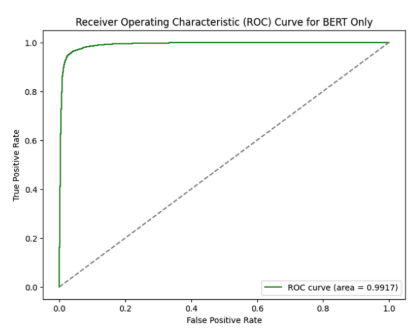
\includegraphics[width=\textwidth]{image/roc_curve_BERT.png}
      \caption{BERT Model}
      \label{fig:roc_curve_bert}
    \end{subfigure}
    \hfill
    \begin{subfigure}[b]{0.3\textwidth}
      \centering
      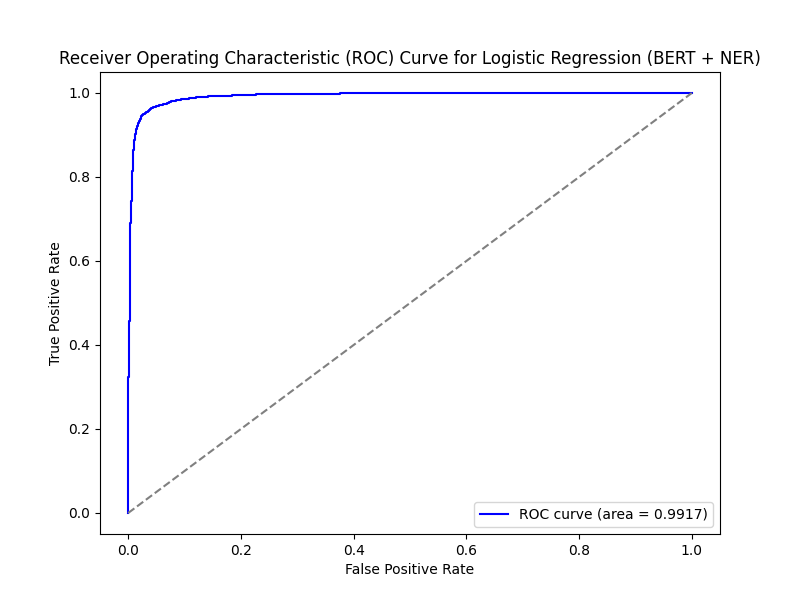
\includegraphics[width=\textwidth]{image/roc_curve_BERT_NER.png}
      \caption{Logistic Regression with NER}
      \label{fig:roc_curve_bert_ner}
    \end{subfigure}
    \hfill
    \begin{subfigure}[b]{0.3\textwidth}
      \centering
      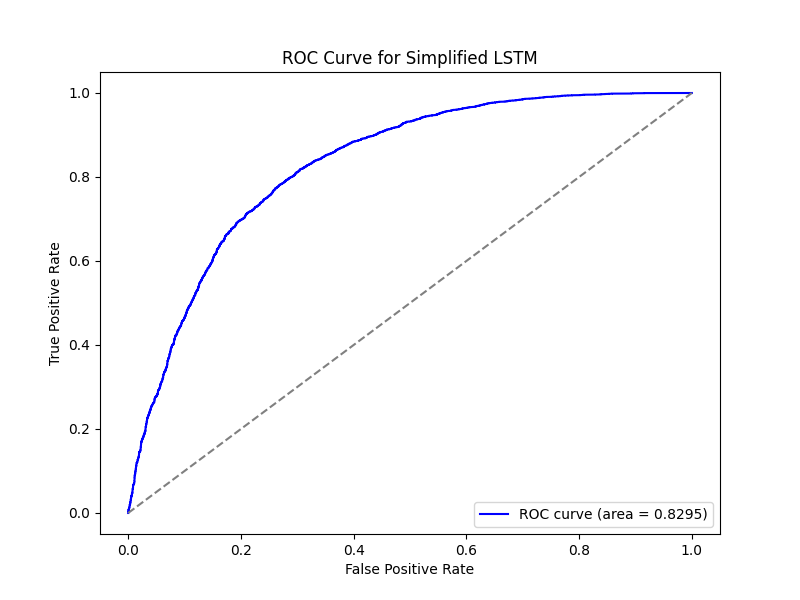
\includegraphics[width=\textwidth]{image/roc_curve_lstm.png}
      \caption{LSTM Model}
      \label{fig:roc_curve_lstm}
    \end{subfigure}
    \caption{Receiver Operating Characteristic (ROC) curves for different models.}
    \label{fig:roc_curve}
\end{figure}

\section{Related Work}

\textbf{Fake News Detection Using Deep Learning Models} \cite{hu2022deep}
This paper explores the use of deep learning architectures, particularly CNNs and RNNs for fake news classification. It highlights the effectiveness of word embeddings in capturing linguistic nuances. 
Compared to their study, our approach will leverage transformer-based models like BERT and extend the classification work by incorporating stance detection into our system.

\textbf{BERT for Fact-Checking and Misinformation Detection} \cite{anggrainingsih2025evaluating}
This study fine-tunes BERT on fact-checking datasets and shows significant performance gains in identifying false claims. 
Our work will build on their use of BERT, but we will also extend it by integrating additional features such as sensationalism detection and source credibility analysis for evaluating contextual cues and maintaining the robustness of fake news classification.

\textbf{Stance Detection for Fake News Identification} \cite{li2022brief}
This research focuses on stance detection to evaluate whether an article supports or contradicts established facts. 
Our approach will extend this work by combining stance detection with linguistic pattern analysis and NER.

\textbf{Social Context and Fake News Propagation} \cite{chen2025enhancing}
This paper investigates how fake news spreads on social media, leveraging user interactions and network analysis. 
While our work will focus on textual credibility analysis, their insights on social media propagation may inform our model extensions.

\textbf{Hybrid Models for Fake News Classification} \cite{mostafa2024modality}
This paper presents a hybrid approach combining linguistic analysis, user features, and propagation dynamics. 
Our model differs by placing greater emphasis on source credibility assessment and stance detection in order to enhance classification through deeper textual understanding rather than propagation signals.

\section{Division of Labor}

\noindent\textbf{Yongbo Chen:}
\begin{itemize}[noitemsep,topsep=0pt]
    \item Implementation of text preprocessing and feature extraction pipeline (Pipeline 1 \& 2)
    \item Development and evaluation of LSTM baseline model (LSTM part of Evaluation 2)
    \item Integration of stance detection module (Evaluation 3)
\end{itemize}

\noindent\textbf{Nazmun Nahar Khanom:}
\begin{itemize}[noitemsep,topsep=0pt]
    \item Implementation of BERT-based classification model (Pipeline 3)
    \item Development of NER component
    \item Implementation and evaluation of Logistic Regression baseline
\end{itemize}

\section{Timeline}

\textbf{Week 1 (9-15 April):} Completed text preprocessing, feature extraction methods, initial BERT classification model setup, and initial accuracy evaluations.

\textbf{Week 2 (16-22 April):} Completed Named Entity Recognition (NER), stance detection, introduced cross-validation to address potential overfitting, and continued baseline comparisons.

\textbf{Week 3 (23-29 April):} Finalize comprehensive evaluations, detailed baseline comparison analysis, and finalize project report.





\bibliographystyle{acl_natbib}
\bibliography{references}


\end{document}
